\documentclass[10pt]{article}
\usepackage{titlesec}
\usepackage{geometry}
\geometry{verbose,tmargin=.9in,bmargin=.9in,lmargin=1.0in,rmargin=1.0in}
\usepackage{amsmath,amsfonts,amsthm,amssymb}
\usepackage{url}
\usepackage{color}
\usepackage[usenames,dvipsnames,svgnames,table]{xcolor}
\usepackage[colorlinks=true, linkcolor=red, urlcolor=blue, citecolor=gray]{hyperref}
\usepackage{float}
\usepackage{caption}
\usepackage{subcaption}
\usepackage{graphicx}
\usepackage{wrapfig}
\usepackage{booktabs}
\usepackage{longtable}
\usepackage{enumerate}
\usepackage{multicol}
\usepackage{etoolbox}
\newcommand{\bs}[1]{\boldsymbol{#1}}
\newcommand{\bv}[1]{\mathbf{#1}}
\usepackage{listings}

\definecolor{nyuDarkPurple}{HTML}{330662}
\definecolor{nyuOfficialPurple}{HTML}{57068c}

\newcommand{\spara}[1]{\vspace{.5em}\noindent {\large\sffamily\textcolor{nyuOfficialPurple}{#1}}}
\titleformat{\section}[hang]{\Large\sffamily\color{nyuDarkPurple}}{\thesection}{1em}{}
\titleformat{\subsection}[hang]{\large\sffamily\color{nyuDarkPurple}}{\thesection}{1em}{}
\titleformat{\subsubsection}[hang]{\normalsize\sffamily\color{gray}}{\thesection}{1em}{}

\usepackage{fancyhdr}
\pagestyle{fancy}
\lhead{
\includegraphics[width=4cm]{tandon_long_color.eps}}
\rhead{\thepage}
\pagenumbering{gobble}

\setcounter{secnumdepth}{0}

% math commands
\DeclareMathOperator{\R}{\mathbb{R}}
\newcommand{\E}{\mathbb{E}}

\begin{document}
	
\begin{center}
	\normalsize
	New York University Tandon School of Engineering
	
	Computer Science and Engineering
	\medskip
	
	\large
	CS-UY 4563: Written Homework 2. 
	
	Due Tuesday, February 18th, 2020, 11:59pm.
	\medskip
	
	\normalsize 
	\noindent \emph{Collaboration is allowed on this problem set, but solutions must be written-up individually. Please list the names of any collaborators at the top of your solution set, or write ``No Collaborators" if you worked alone.}
	\medskip
\end{center} 

\subsection{Problem 1: Practice Framing a Multiple Regression Problem (10pts)}
 An online retailer like Amazon wants to determine which products to promote based on reviews. They only want to promote products that are likely to sell. For each product, they have past sales as well as reviews. The reviews have both a numeric score (from 1 to 5) and text.
 
\begin{enumerate}[(a)]
	\item (2pts) To formulate this as a machine learning problem, suggest a target variable that the online retailer could use.
	
	\color{blue}
	One target variable could be the number of sales per day of the product. Or better, the likelihood a customer buys the product after a visit to the product page (places like Amazon collect that info.). Students might also have suggestions which take price into account -- we might want to recommend products which make more money per sale. 
	\color{black}
	
	\item (3pts)  For the predictors of the target variable, a data scientist suggests to combine each review's numeric score with the frequency of occurrence of words that convey judgement like ``bad'', ``good'', ``broke'', or ``bargain''. The data scientist would like to use these features in a linear model.
	
	Describe one logical way to build feature vectors for each product. Think about normalization here!
	
	\color{blue}
	\textbf{Note: Make sure they describe features for each product, not for individual reviews!}
	
	Our first column could simply include the average rating for the product. There are other answers that would be fine here too: for example, you could have 5 separate columns which separately encode the percentage of review scores which are $1,2,3,4,5$ for the product. 
	
	For the word data, one reasonable option is to create a feature column for each of the selected words which convey judgement. I.e. we would have a column for ``bad'', ``good'', ``bargain'' etc. In each column, in the row for a particular product, we could include the number of times the word appears in all reviews for that product. It's probably a good idea to normalize for the total number of reviews or total length of reviews for the product (e.g. use word frequency divided by total number of reviews.) Otherwise, very heavily reviewed products might have more ``good'' words than less reviewed products, even if the heavily reviewed product is rated more poorly overall.
	\color{black}
		

	
	\item (2pts) Suppose that some reviews have a numeric score from 1 to 5 and others have a score from 1 to 10. How would change your features?
	
		\color{blue}
	We would likely want to adjust things so all reviews are on the same scale -- an easy way to do this is to multiply the numerical score for any review using a $1-5$ rating by 2. Then, when we average scores  to form our  first column, we would simply include the average rating for the product on the $1-10$ scale.
	\color{black}
	
	\item  (3pts) Now suppose the reviews have either:  a score from 1 to 5;  a rating that is simply good or bad; or no numeric rating at all. How would you change your features?
		\color{blue}
		
	Again, there are a lot of possible answers here. One option is to to translate ``good'' and ``bad'' to a numerical score on our $1-10$ scale (e.g. good = 8, bad = 3) and include in the average as above.
	Another option is to do some sort of $1$-hot encoding. For example, we could have $12$ columns for every possible score $1,\ldots, 10, \text{good}, \text{bad}$. In each of those columns we put the proportion of the reviews for each product that was given that score.
		\color{black}
\end{enumerate}

\newpage

\subsection{Problem 2: Thinking About Data Transformations (10pts)}
You are trying to fit a multiple linear regression model for a given data set. You have already transformed your data by appending a column of all ones, which resulted in a final data matrix:
\begin{align*}
X = \begin{bmatrix}
1 & x_{1,1} & x_{1,2} & \ldots & x_{1,d} \\
1 & x_{2,1} & x_{2,2} & \ldots & x_{2,d} \\
\vdots & \vdots & & \vdots\\
1 & x_{n,1} & x_{n,2} & \ldots & x_{n,d} \\
\end{bmatrix}
\end{align*}
However, your model does not seem to be working well. It obtains poor loss in both training and test. 
\begin{enumerate}[(a)]
	\item (4pts) A friend suggests that you should try mean centering your data columns. In other words, for each $i$, compute the column mean $\bar{x}_i = \frac{1}{n}\sum_{j=1}^n x_{i,j}$ and subtract $\bar{x}_i$ from every entry in column $i$. Note that we won't mean center the first column, as doing so would set the 1s to 0s.
	Using Python broadcasting you might mean center by running:
	\begin{lstlisting}
	T = X[:,1:]
	X[:,1:] = T - np.mean(T,axis=0)
	\end{lstlisting}
	Do you expect your friend's suggestion to improve the performance of the linear model. Will it help in all cases? Some cases? No cases?
	
	\color{blue}
	\textbf{Note: students can give a much less formal answer, as long as it's clear they get the point.}
	
	Mean centering is unlikely to help in any case, at least for any of the standard loss function we have considered. In particular, it won't make a difference for any loss of the form $L(X\beta - y)$, where $X$ is the data matrix, $y$ is the vector of $n$ targets, and $\beta$ is a parameter vector.  Below we explain why:
	
	Let $\bar{X}$ denote our matrix with mean centered columns. Denote the $i^\text{th}$ column of $\bar{X}$ by $\bar{X}_i$. Clearly $\bar{X}_i = X_i - c_i \vec{1}$ for some constant $c_i$ (in this case $c_i = \bar{x}_i)$. Here $\vec{1}$ is the all ones vector. 
	
	Now, given any $\beta$, we claim that there always exists some $\bar{\beta}$ such that $X\beta = \bar{X}\bar{\beta}$. Specifically set $\bar{\beta}_i = {\beta}_i$ for all $i > 1$ and set $\bar{\beta}_1 = \beta_1 + \sum_{i=2}^n c_i$. At the same time, given any  $\bar{\beta}$, there is always some $\beta$ such that $X\beta = \bar{X}\bar{\beta}$. Specifically set ${\beta}_i = \bar{\beta}_i$ for all $i > 1$ and set ${\beta}_1 = \bar{\beta}_1 - \sum_{i=2}^n c_i\bar{\beta}_i$.
	
	We conclude that for any loss of the form stated above, 
	\begin{align*}
	\min_\beta L(X,y,\beta) = 	\min_\beta L(\bar{X},y,\beta).
	\end{align*}
	So scaling certainly won't help improve training loss. It's possible it leads to some small difference in test loss, but its hard too say either way: we don't expect the test loss to be small if training loss isn't. 
	\color{black}
	
	\item (4pts)  Another friend suggests normalizing your data columns to have unit standard deviation. In other words for each $i$, compute the column standard deviation $\sigma_i = \sqrt{\frac{1}{n}\sum_{j=1}^n (x_{i,j} - \bar{x}_i)^2}$ and \emph{divide} every column by $\sigma_i$. 
	Using Python broadcasting you might run:
	\begin{lstlisting}
	T = X[:,1:]
	X[:,1:] = T/np.std(T,axis=0)
	\end{lstlisting}
	Do you expect your friends suggestion to improve the performance of the linear model. Will it help in all cases? Some cases? No cases?
	
	\color{blue}
	The argument is essentially the same as above. Let $\bar{X}$ be our data set with each column multiplied by $c_i$. For 
	any $\beta$ there is some $\bar{\beta}$ such that $X\beta = \bar{X}\bar{\beta}$: set 
	$\bar{\beta}_i = \frac{1}{c_i}\beta_i$ for all $i > 1$. 
	Similarly, for any $\bar{\beta}$ there is some $\beta$ with 
	$X\beta = \bar{X}\bar{\beta}$: 
	set $\beta_i = c_i \bar{\beta}_i$ for all 
	$i > 1$.  Again we conclude that:
	
	\begin{align*}
	\min_\beta L(X,y,\beta) = 	\min_\beta L(\bar{X},y,\beta).
	\end{align*}
	so the transformation cannot improve training loss. 
	
	\color{black}
	
	\item (2pts)  Would your answers to either of the two questions above change if you were fitting the model with $\ell_2$ regularization? In other words, instead of minimizing the squared loss $L(\bs{\beta}) = \|\bv{y} - \bv{X}\bs{\beta}\|_2^2$ alone, you were minimizing $L(\bs{\beta}) + \lambda\|\bs{\beta}\|_2^2$. 
	
	\color{blue}
	\textbf{Again, no need for them to be super formal here. They just need to identify that regularization changes things.}
	
	Under $\ell_2$ regularization, it's possible that both mean centering or scaling by standard deviation could improve performance. It's also possible they could make things worse, or do nothing at all. For example, suppose we have a column $i$ in $X$ which has very small standard deviation. Scaling that column by the inverse of the standard deviation will effectively allow our regularized solution to  place more mass at $\beta_i$. If that column is a good predictor for $y$, this change could substantial improve test loss. 
	\color{black}

\end{enumerate}

\newpage
\subsection{Problem 3: Practice With Gradients (10pts)}
For $\bv{X} \in \R^{n\times d}$ and target vector $\bv{y} \in \R^n$, consider fitting a linear model of the form:
\begin{align*}
f_{\bs{\beta}}(\bv{x}) = \bv{X}\bs{\beta}
\end{align*}
under the so-called $\ell_p$ loss: $L_p(\bs{\beta}) = \|\bv{y} - f_{\bs{\beta}}(\bv{x})\|_p^p$. Here $\|\cdot \|_p^p$ denotes the $\ell_p$ norm raised to the $p$ power. I.e. for any even integer $p = 2,4,6, \ldots$
\begin{align*}
\|\bv{z}\|_p^p = \sum_{i=1}^n z_i^p
\end{align*}

\begin{enumerate}[(a)]
	\item (5pts)  Derive an expression for $\nabla g(\bv{z})$ where $g(\bv{z}) = \|\bv{z}\|_p^p$. 
	
	\color{blue}
	We have that $\partial g / \partial z_i = pz_i^{p-1}$. So if we stack all of the partial derivatives into a column vector we have: $\nabla g(\bv{z}) = p \bv{z}^{p-1}$ where $\bv{z}^{p-1}$ denotes raising every entry in the vector $\bv{z}$ to the $p-1$ power.
	\color{black}
	
	\item (5pts -- I would give 3pts if they get the expression correct, 2pts for correct justification. Some will just pattern match from class and guess the right thing.) Derive an expression for $\nabla L_p(\bs{\beta})$. \textbf{Hint:} Use chain rule.
	
	\color{blue}
	Let $h(\bv{z}) = \|\bv{y} - \bv{z}\|_p^p$ for some fixed vector $\bv{y}$. Using the same argument as in part (a), we have that $\nabla h(\bv{z}) = - p \left(\bv{y} - \bv{z}\right)^{p-1}$. Then we can apply the multivariate chain rule from class, and in particular the special case where the input of a function is multiplied by a matrix. 
	
	Specifically, we have that $L_p(\bs{\beta}) = h(\bv{X}\bs{\beta})$. So $\nabla L_p(\bs{\beta})  = \bv{X}^T \nabla h(\bv{X}\bs{\beta}) = -p \bv{X}^T\left(\bv{y} - \bv{X}\bs{\beta}\right)^{p-1}$ where again the power denotes an entrywise operation.
	\color{black}
\end{enumerate}

\newpage

\subsection{Problem 4: Piecewise Linear Regression via Feature Transformations (15pts)}
Your goal is to fit a \emph{piecewise} linear model to a single variate dataset of the form $(x_1, y_1), \ldots, (x_n, y_n)$ where all values are scalars. We will only use two pieces. In other words, for some known value $\lambda$, 
\begin{align*}
f(x_i) = \begin{cases}
a_1 + s_1x_i & \text{ for $x_i < \lambda$}\\ 
a_2 + s_2x_i & \text{ for $x_i \geq \lambda$}
\end{cases}
\end{align*}
with the additional \textbf{constraint} that $a_1 + s_1\lambda = a_2 + s_2\lambda$. This constraint ensures that our two linear models actually ``meet'' at $x = \lambda$, which means we get a continuous prediction function.

For example, when $\lambda = 100$, a piecewise linear fit for our MPG data might look like:
\begin{figure}[H]
	\centering
	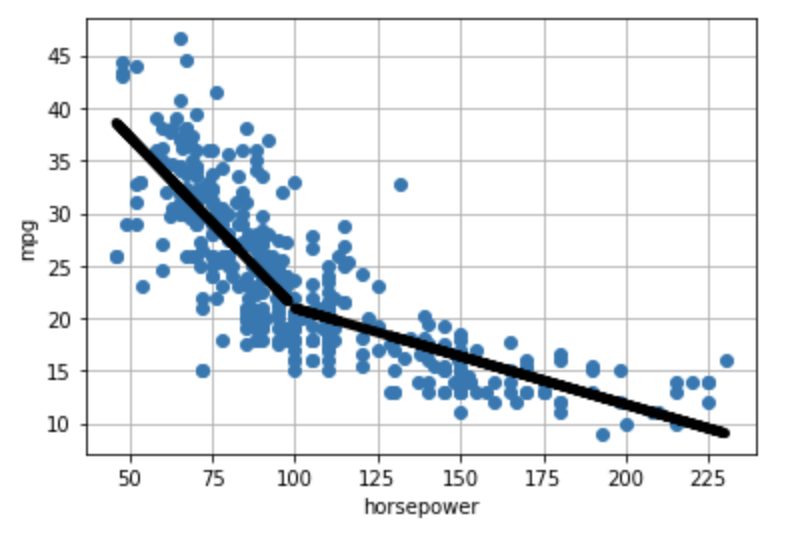
\includegraphics[width=.4\textwidth]{piecewise_fit.png} 
\end{figure}

\begin{enumerate}[(a)]
	\item (2pts) Show that this model is equivalent to the following \textbf{unconstrained} model:
	\begin{align*}
	f(x_i) = \begin{cases}
		a_1 + s_1x_i & \text{ for $x_i < \lambda$}\\ 
		a_1 + s_1 \lambda - s_2 \lambda + s_2x_i & \text{ for $x_i \geq \lambda$}
	\end{cases}
	\end{align*}
	
	\color{blue}
	From our constraint, we always have that $a_2 = a_1 + s_1\lambda  - s_2\lambda$. So we can eliminate the $a_2$ parameter: it is completely determined by the other model parameters. Simply replacing $a_2$ in $f(x_i)$ with $a_1 + s_1\lambda  - s_2\lambda$ gives the alternative formulation. 
	\color{black}
	
	\item (7pts) Show how to fit an optimal $f$ under the squared loss using an algorithm for multiple linear regression. In particular, your approach should:
	\begin{itemize}
		\item Transform the input data to form a data matrix $\bv{X}$ with multiple columns.
		\item Use a multiple regression algorithm to find the $\bs{\beta}$ which minimizes $\|\bv{y} - \bv{X}\bs{\beta}\|_2^2.$
		\item Extract from the optimal $\bs{\beta}$ optimal values for $a_1, s_1, s_2$. 
	\end{itemize} 
	You need to describe 1) a correct data transformation and 2) a correct mapping from $\bs{\beta}$ to $a_1, s_1, s_2$. 
	\textbf{Note that in our model $\lambda$ is known. It is not a model parameter which needs to be optimized.}
	
	\color{blue}
	Construct $\bv{X}$ as follows:
	\begin{itemize}
		\item First column equal to $\vec{1}$. 
		\item Second column equal to $x_i$ for any position $i$ such that $x_i < \lambda$. Otherwise, equal to $\lambda$ for any position $i$ such that $x_i \geq \lambda$.
		\item Third column equal to $0$ for any position $i$ such that $x_i < \lambda$.  Otherwise, equal to $x_i - \lambda$ for any position $i$ such that $x_i \geq \lambda$.  
	\end{itemize}

	Now consider $\bv{X}\bs{\beta}$. With some thought we see that the $i^\text{th}$ entry of this vector is equal to $f(x_i)$ with parameters $a_1 = \bs{\beta}_1$, $s_1 = \bs{\beta}_2$, and $s_2 = \bs{\beta}_3$.
	\color{black}
	
	\item (6pts -- I would give most of the credit if they faithfully implemented their solution to part (b). I would give full credit if they did so and it produced a reasonable solution. If the solution looks very wrong (i.e. clearly a bad fit) you can take 3 pts off -- they should know to sanity check their results and adjust if they look wrong.)
	
	 Implement your algorithm in Python and apply it to the dataset from \texttt{demo\_auto\_mpg.ipynb}. Produce a piecewise linear fit for MPG as a function of Horsepower using the value $\lambda = 100$. Plot the result. You can attach a Jupyter notebook to your submission, or simply include the printed code and plot. 
	
	\color{blue}
	See my solution in \texttt{part\_4\_soln.ipynb}.
	\color{black}
	
	\item (\textbf{5pts bonus}) Modify your approach to handle the case when $\lambda$ is unknown. Again obtain a fit for MPG vs. horsepower. What value of $\lambda$ gives the optimal fit? Include any modified code and a plot of your result.
	
	\color{blue}
	Easiest way to do this is by brute forcing over a grid of possible values of $\lambda$. For students who are struggling with the mathematical part but more comfortable with coding, you can give a hint to suggest this -- e.g. ask if any tools from the first lab might come in handy. It's a good way for them to make up some points.
	\color{black}
\end{enumerate}






\end{document}